%*************************************
% บทที่ 2
%*************************************
\chapterTitle{2}{แนวคิด ทฤษฎี และงานวิจัยที่เกี่ยวข้อง}
\providecommand{\cmark}{\ensuremath{\checkmark}}
\providecommand{\xmark}{\ensuremath{\times}}
\vspace{0.2in}
\hspace*{1.3em}
ในการวิเคราะห์ ออกแบบ และพัฒนาระบบปัญญาประดิษฐ์แชทบอทสำหรับองค์กร กรณีศึกษา บริษัท ฮาร์ทวอมมิ่ง จำกัด คณะผู้จัดทำได้ศึกษาค้นคว้าแนวคิด ทฤษฎี เทคโนโลยี ซอฟต์แวร์ และงานวิจัยที่เกี่ยวข้อง เพื่อใช้เป็นกรอบแนวทางและหลักการทางวิศวกรรมซอฟต์แวร์ในการพัฒนาระบบ โดยแบ่งเนื้อหาออกเป็นหัวข้อสำคัญตามลำดับ ดังนี้:

\section{ทฤษฎีการค้นคืนข้อมูลเสริมด้วยปัญญาประดิษฐ์ (Retrieval-Augmented Generation: RAG)}
\hspace*{1.3em}
แม้ว่าโมเดลภาษาขนาดใหญ่ (Large Language Models: LLM) ในปัจจุบันจะมีความสามารถในการประมวลผลและสร้างภาษาธรรมชาติได้อย่างยอดเยี่ยม ทว่าโมเดลภาษาทั่วไปยังมีข้อจำกัดสำคัญ 2 ประการ คือ 1) อาการภาพหลอนของข้อมูล (Hallucination) ซึ่งโมเดลอาจสร้างคำตอบที่ดูน่าเชื่อถือแต่ข้อเท็จจริงผิดพลาด และ 2) ขาดข้อมูลบริบทเฉพาะขององค์กร เนื่องจากโมเดลถูกฝึกสอนด้วยชุดข้อมูลสาธารณะ ไม่ได้รับรู้ข้อมูลระเบียบ เอกสาร หรือสินค้าเฉพาะของ บริษัท ฮาร์ทวอมมิ่ง จำกัด

\hspace*{1.3em}
แนวคิดการค้นคืนข้อมูลเสริมด้วยปัญญาประดิษฐ์ (Retrieval-Augmented Generation: RAG) จึงถูกคิดค้นขึ้นเพื่อแก้ปัญหาดังกล่าว โดยเป็นสถาปัตยกรรมที่ผสานระหว่างสองส่วนหลัก คือ ระบบการค้นคืนสารสนเทศ (Information Retrieval: IR) และโมเดลกำเนิดภาษา (Generative Model) มีขั้นตอนการทำงาน 3 ระยะสำคัญ ได้แก่: 1) ขั้นตอนการค้นคืน (Retrieval Phase) ระบบแปลงคำถามเป็นเวกเตอร์และสืบค้นท่อนข้อความที่มีความคล้ายคลึงสูงสุด 2) ขั้นตอนการเสริมบริบท (Augmentation Phase) นำข้อความที่ค้นได้มารวมเข้ากับ System Prompt และ 3) ขั้นตอนการสร้างคำตอบ (Generation Phase) โมเดลภาษาขนาดใหญ่สังเคราะห์คำตอบที่ถูกต้องตรงตามเอกสารต้นฉบับ

\subsection{การแบ่งเอกสารและการแปลงเป็นเวกเตอร์ (Document Chunking \& Vector Embeddings)}
\hspace*{1.3em}
เอกสารต้นฉบับ เช่น คู่มือสินค้า duit, นโยบายการคืนสินค้า thumb toe หรือระเบียบการทำงาน จะถูกนำมาทำความสะอาดและแบ่งเป็นส่วนย่อย ๆ (Chunk Size ประมาณ 500-1,000 ตัวอักษร พร้อม Overlap 100 ตัวอักษร) เพื่อรักษาความต่อเนื่องของบริบท จากนั้นแต่ละท่อนข้อความจะถูกส่งเข้าสู่โมเดล Embedding เพื่อแปลงเป็นเวกเตอร์ตัวเลขหลายมิติ (High-Dimensional Dense Vector)

\subsection{ฐานข้อมูลเวกเตอร์ (Vector Database) และการวัดความคล้ายคลึง}
\hspace*{1.3em}
โครงงานนี้เลือกใช้ ChromaDB ร่วมกับโมเดล FastEmbed ซึ่งเป็นฐานข้อมูลเวกเตอร์แบบโอเพนซอร์สที่มีประสิทธิภาพสูง สามารถคำนวณระยะห่างระหว่างเวกเตอร์ของคำถามกับเวกเตอร์เอกสารโดยใช้การวัดความคล้ายคลึงแบบโคไซน์ (Cosine Similarity) หรือระยะห่างแบบยุคลิด (Euclidean Distance) ทำให้ระบบสามารถค้นหาข้อมูลที่ตรงความหมายได้แม้ผู้ใช้จะใช้คำศัพท์ที่ไม่ตรงกับคีย์เวิร์ดในเอกสารโดยตรง

\section{โมเดลภาษาขนาดใหญ่และการประมวลผลภาษาธรรมชาติ (LLM \& NLP)}

\subsection{โมเดลภาษาขนาดใหญ่ Google Gemini}
\hspace*{1.3em}
ระบบ OrgChat AI เลือกใช้บริการโมเดล Google Gemini ซึ่งพัฒนาบนพื้นฐานสถาปัตยกรรม Transformer ที่มีความสามารถระดับ Multimodal คือเข้าใจทั้งข้อความ รูปภาพ และโค้ด มีความสามารถในการประมวลผลภาษาไทยได้อย่างเป็นธรรมชาติ เข้าใจไวยากรณ์ สำนวนภาษา และบริบทการสนทนาทางธุรกิจของคนไทยได้อย่างยอดเยี่ยม

\subsection{การตัดคำและการประมวลผลภาษาไทย (Thai Tokenization)}
\hspace*{1.3em}
เนื่องจากภาษาไทยเป็นภาษาที่เขียนคำติดต่อกันโดยไม่มีการเว้นวรรคระหว่างคำ ระบบจึงต้องประยุกต์ใช้เทคนิคการตัดคำภาษาไทยและการจัดการพยางค์ เพื่อให้กระบวนการสร้างเวกเตอร์และวิเคราะห์เจตนาของผู้ใช้ (Intent Classification) มีความถูกต้อง ไม่เกิดการตัดคำผิดความหมาย เช่น การแยกชื่อสินค้าเฉพาะ หรือรหัส SKU

\subsection{วิศวกรรมคำสั่ง (Prompt Engineering)}
\hspace*{1.3em}
การกำหนด System Instructions และ Few-Shot Prompts เพื่อควบคุมบุคลิกของแชทบอทให้ตอบคำถามอย่างสุภาพ มืออาชีพ ตรงประเด็น และกำหนดเงื่อนไขความปลอดภัย (Safety \& Guardrails) ให้แชทบอทตอบคำถามเฉพาะข้อมูลที่มีอยู่ในคลังความรู้ของบริษัท ฮาร์ทวอมมิ่ง จำกัด เท่านั้น

\section{ทฤษฎีการประมวลผลภาพดิจิทัลและการรู้จำอักขระด้วยแสง (Digital Image Processing \& OCR)}
\hspace*{1.3em}
การจัดการเอกสารทางการเงิน เช่น สลิปโอนเงินผ่าน Mobile Banking และใบเสร็จรับเงิน จำเป็นต้องอาศัยเทคโนโลยีการประมวลผลภาพดิจิทัลและการรู้จำอักขระด้วยแสง (OCR) เพื่อแปลงภาพถ่ายให้เป็นข้อมูลดิจิทัลที่คอมพิวเตอร์ประมวลผลได้ โดยมีกระบวนการเตรียมภาพสำคัญ ได้แก่: 1) การแปลงภาพเป็นระดับสีเทา (Grayscale Conversion) เพื่อลดมิติข้อมูลสี 2) การปรับภาพเป็นไบนารี (Otsu's Thresholding \& Binarization) แยกตัวอักษรออกจากพื้นหลัง 3) การลดสัญญาณรบกวน (Denoising) ด้วย Gaussian Blur และ Median Filtering และ 4) การปรับแก้ความเอียงของเอกสาร (Deskewing) ด้วย Hough Transform

\subsection{เทคโนโลยีการรู้จำอักขระ (Optical Character Recognition: OCR)}
\hspace*{1.3em}
ระบบใช้ Google Cloud Vision API เป็นเครื่องมือหลักในการตรวจจับตำแหน่งข้อความ (Text Detection) และอ่านตัวอักษรทั้งภาษาไทย ภาษาอังกฤษ และตัวเลข โดยมีความแม่นยำสูงแม้ภาพจะมีความละเอียดต่ำ พร้อมรองรับ Tesseract OCR เป็นระบบสำรอง (Fallback Engine)

\subsection{การสกัดข้อมูลด้วยนิพจน์ปกติ (Regular Expression: Regex Extraction)}
\hspace*{1.3em}
ข้อความดิบที่ได้จาก OCR จะถูกส่งเข้าสู่ระบบประมวลผลข้อมูล เพื่อสกัดฟิลด์สำคัญ ได้แก่: รูปแบบวันที่และเวลา (DD/MM/YYYY, HH:MM), จำนวนเงินและทศนิยม (\verb|^[0-9,]+\.[0-9]{2}\$|), ชื่อธนาคารผู้โอน/ผู้รับโอน, เลขที่บัญชี และรหัสอ้างอิงธุรกรรม (Transaction ID) เพื่อนำไปจัดหมวดหมู่และลงบัญชี

\section{ทฤษฎีสถาปัตยกรรมซอฟต์แวร์และการพัฒนาเว็บแอปพลิเคชัน}

\subsection{สถาปัตยกรรมที่ขับเคลื่อนด้วยเหตุการณ์ (Event-Driven Architecture)}
\hspace*{1.3em}
ระบบแชทบอททำงานในรูปแบบรอรับเหตุการณ์ (Event Listener) เมื่อผู้ใช้งานส่งข้อความ รูปภาพ หรือกดยื่นใบลาผ่าน LINE ระบบจะสร้าง Webhook Event ส่งมายังเซิร์ฟเวอร์แบบ Asynchronous ทำให้เซิร์ฟเวอร์สามารถรองรับการทำงานพร้อมกันของผู้ใช้หลายคนได้อย่างมีเสถียรภาพ

\subsection{สถาปัตยกรรมแยกส่วนหน้าและส่วนหลัง (Client-Server Architecture)}
\hspace*{1.3em}
เว็บแอปพลิเคชันถูกออกแบบให้ส่วนแสดงผล (Frontend) ซึ่งสร้างด้วย HTML5, CSS3 และ JavaScript ทำงานแยกจากส่วนตรรกะการประมวลผล (Backend) ที่เขียนด้วยภาษาไพทอน โดยสื่อสารกันผ่าน RESTful API ในรูปแบบมาตรฐาน JSON ทำให้ง่ายต่อการบำรุงรักษาและขยายระบบในอนาคต

\subsection{เว็บเฟรมเวิร์ก Flask (Python)}
\hspace*{1.3em}
Flask เป็น Microframework สำหรับภาษาไพทอนที่มีความยืดหยุ่นสูง น้ำหนักเบา และมีประสิทธิภาพการประมวลผลที่รวดเร็ว เหมาะสำหรับการสร้างทั้ง Web Application และ RESTful Web Services

\begin{figure}[htbp]
\centering
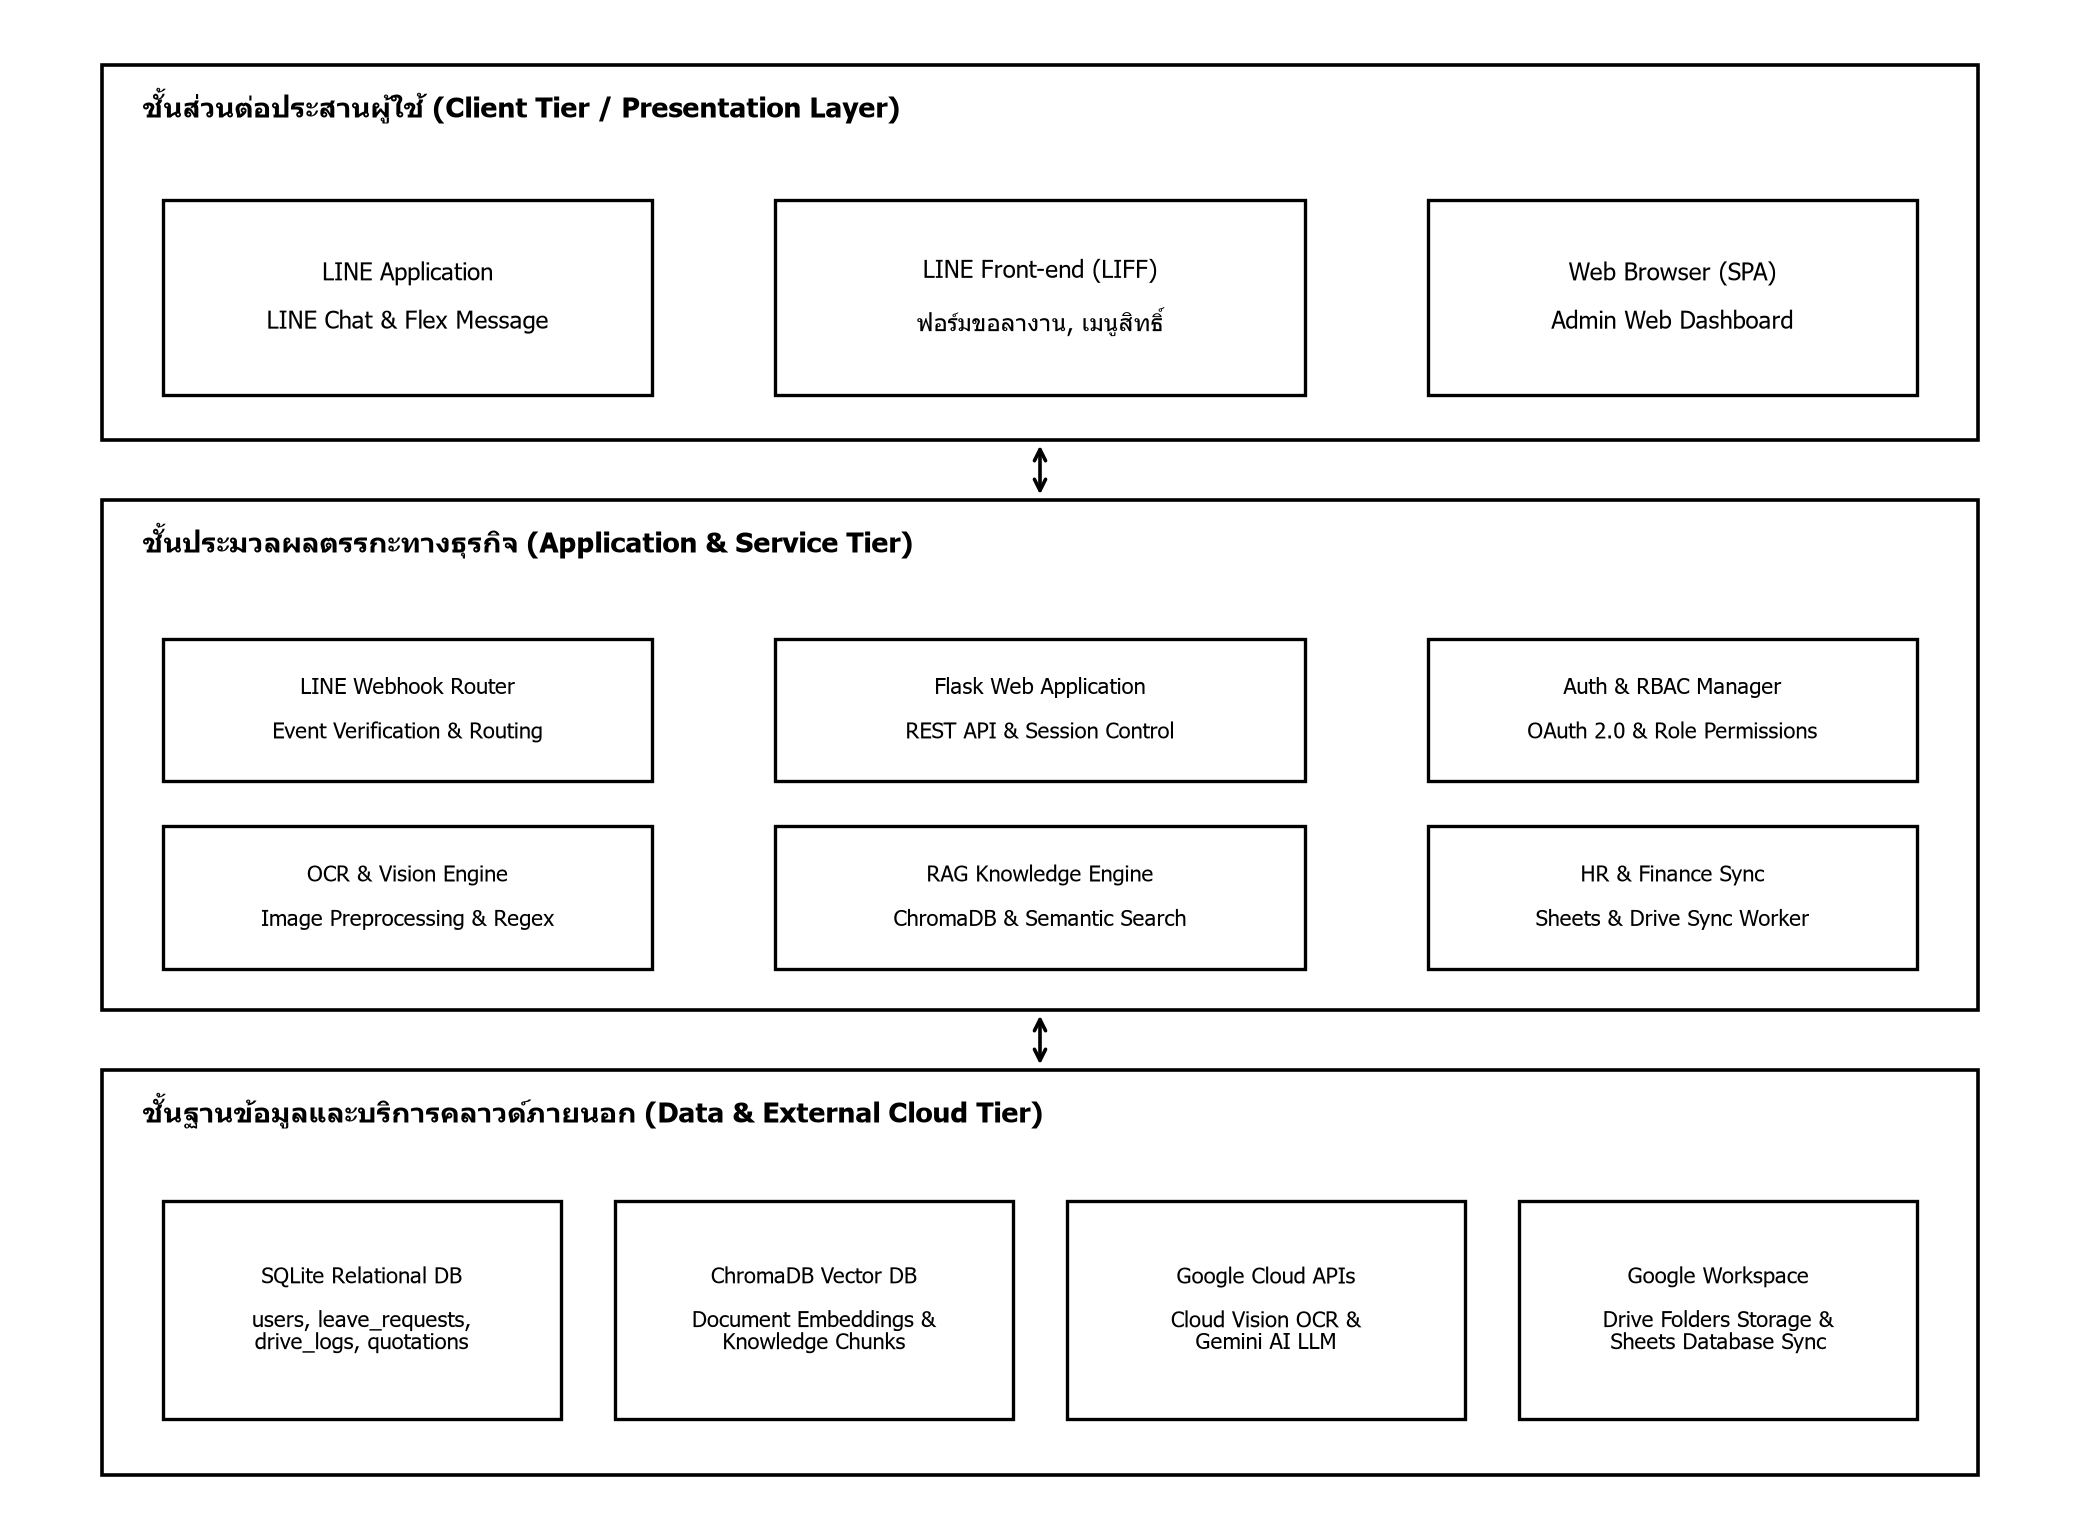
\includegraphics[width=0.95\textwidth]{Image/fig2_1_architecture.png}
\caption{สถาปัตยกรรมระบบปัญญาประดิษฐ์แชทบอทสำหรับองค์กร (System Architecture Diagram)}
\label{fig2:architecture}
\end{figure}

\section{แพลตฟอร์มและการเชื่อมต่อ LINE (Messaging API \& LIFF)}

\subsection{LINE Messaging API}
\hspace*{1.3em}
เป็นชุดเครื่องมือที่ช่วยให้นักพัฒนาสามารถส่งข้อความแบบสองทาง (Two-way communication) ระหว่างผู้ใช้งาน LINE กับเซิร์ฟเวอร์ของระบบ โดยเซิร์ฟเวอร์จะรับ Webhook Event ผ่าน HTTPS POST request พร้อมการตรวจสอบความถูกต้องของลายเซ็นดิจิทัล (X-Line-Signature) ด้วยอัลกอริทึม HMAC-SHA256 เพื่อป้องกันการปลอมแปลงคำขอ

\subsection{LINE Front-end Framework (LIFF)}
\hspace*{1.3em}
เป็นแพลตฟอร์มสำหรับแสดงผลเว็บแอปพลิเคชันภายในแอปพลิเคชัน LINE ช่วยให้ผู้ใช้สามารถเปิดหน้าจอเว็บ เช่น หน้าฟอร์มยื่นคำขอลางาน หรือหน้าระบบรายงาน โดยไม่ต้องออกจากแอป LINE

\subsection{LINE Flex Message}
\hspace*{1.3em}
สถาปัตยกรรมการแสดงผลข้อความในรูปแบบการ์ดที่สามารถจัดวางโครงสร้างคล้ายหน้าเว็บ (CSS Flexible Box) สามารถกำหนดสี ขนาดตัวอักษร การจัดวางปุ่มกด Call-to-Action (เช่น ปุ่ม "อนุมัติ" / "ปฏิเสธ" การลา)

\section{ทฤษฎีการจัดการฐานข้อมูลและสถาปัตยกรรมมัลติเทแนนต์ (Database \& Multi-Tenant)}

\subsection{ทฤษฎีการออกแบบฐานข้อมูลเชิงสัมพันธ์และกระบวนการนอร์มัลไลเซชัน (Database Normalization)}
\hspace*{1.3em}
การออกแบบตารางข้อมูลในระบบ OrgChat AI ผ่านกระบวนการนอร์มัลไลเซชันให้อยู่ในระดับ 3NF (Third Normal Form) เพื่อลดความซ้ำซ้อนของข้อมูล และกำหนดคีย์หลัก (Primary Key) ร่วมกับคีย์นอก (Foreign Key) เพื่อรักษา Referential Integrity

\subsection{คุณสมบัติ ACID ของการทำธุรกรรม (ACID Properties)}
\hspace*{1.3em}
รับประกันคุณสมบัติ Atomicity, Consistency, Isolation และ Durability โดยเฉพาะการตัดโควตาวันลาและการลงบัญชี

\subsection{สถาปัตยกรรมแยกข้อมูลระหว่างองค์กร (Multi-Tenant Data Isolation)}
\hspace*{1.3em}
ใช้โมเดล Shared Database with Tenant-Specific Partitioning โดยทุกตารางข้อมูลหลักจะมีคอลัมน์ \texttt{org\_id} กำกับไว้เพื่อป้องกันการเข้าถึงข้อมูลข้ามองค์กร

\section{ทฤษฎีความปลอดภัยและการควบคุมสิทธิ์การเข้าถึง (Information Security \& RBAC)}

\subsection{การควบคุมการเข้าถึงตามบทบาท (Role-Based Access Control: RBAC)}
\hspace*{1.3em}
ระบบกำหนดสิทธิ์การใช้งานแบ่งตามระดับบทบาทหน้าที่ 5 ระดับ ได้แก่ Super Administrator, Organization Admin, Manager, Employee และ General User ยึดตามมาตรฐาน NIST (2020)

\subsection{ความปลอดภัยของรหัสผ่านและการจัดการเซสชัน}
\hspace*{1.3em}
ใช้ฟังก์ชันแฮชทางเดียว PBKDF2/Bcrypt พร้อม Salt สุ่ม ร่วมกับการจัดการเซสชันที่ปลอดภัย คุกกี้ HttpOnly, Secure และ SameSite

\subsection{การรักษาความสมบูรณ์ของเอกสารและบันทึกตรวจสอบ (File Integrity \& Audit Logging)}
\hspace*{1.3em}
คำนวณค่าแฮช SHA-256 สำหรับไฟล์เอกสารทุกฉบับ พร้อมบันทึกประวัติการกระทำสำคัญลงใน Audit Logs

\section{การเชื่อมต่อบริการคลาวด์ภายนอก (Google Cloud \& Workspace APIs)}

\subsection{Google Drive API}
\hspace*{1.3em}
จัดเก็บไฟล์เอกสารและสลิปแบบแยกโฟลเดอร์ตามปี พ.ศ. และเดือนโดยอัตโนมัติ

\subsection{Google Sheets API}
\hspace*{1.3em}
บันทึกข้อมูลการเงินรายรับ-รายจ่ายเป็นสมุดบัญชีออนไลน์แบบเรียลไทม์

\section{ทฤษฎีการออกแบบส่วนต่อประสานผู้ใช้และการแสดงผลข้อมูลเชิงภาพ (UI/UX \& Data Visualization)}
\hspace*{1.3em}
ยึดหลักการ 10 ประการของ Jakob Nielsen (Usability Heuristics) ร่วมกับการใช้ไลบรารี Chart.js ในการสร้างกราฟแท่ง กราฟวงกลม และกราฟเส้นแสดงสถิติภาพรวมบนแผงควบคุม

\section{ซอฟต์แวร์และเครื่องมือที่ใช้ในการพัฒนา (Development Tools \& Software)}
\hspace*{1.3em}
ในการดำเนินงานจัดทำโครงงานพิเศษนี้ คณะผู้จัดทำได้เลือกใช้เครื่องมือและซอฟต์แวร์มาตรฐานในวิศวกรรมซอฟต์แวร์ ดังนี้:

\noindent\hspace*{1.3em}\textbf{1) Visual Studio Code (VS Code):} โปรแกรมแก้ไขโค้ดหลัก รองรับส่วนขยายสำหรับการเขียนโค้ดภาษา Python, HTML5, CSS และการจัดการสภาพแวดล้อมเสมือน\par\vspace{0.25em}
\noindent\hspace*{1.3em}\textbf{2) Python 3.10+ และ Flask Framework:} ภาษาโปรแกรมและเว็บเฟรมเวิร์กฝั่งเซิร์ฟเวอร์หลัก ใช้ในการจัดการเส้นทาง API, Webhook Handler และการเชื่อมต่อ AI โมเดล\par\vspace{0.25em}
\noindent\hspace*{1.3em}\textbf{3) SQLite และ ChromaDB:} SQLite ใช้สำหรับจัดเก็บข้อมูลเชิงสัมพันธ์ของผู้ใช้งานและองค์กร ขณะที่ ChromaDB เป็นฐานข้อมูลเวกเตอร์ประสิทธิภาพสูงสำหรับระบบ RAG\par\vspace{0.25em}
\noindent\hspace*{1.3em}\textbf{4) Git และ GitHub:} ระบบควบคุมเวอร์ชันซอฟต์แวร์แบบกระจายศูนย์ ใช้ในการบันทึกประวัติการพัฒนาโค้ดและทำงานร่วมกันในทีม\par\vspace{0.25em}
\noindent\hspace*{1.3em}\textbf{5) Figma:} เครื่องมือออกแบบส่วนต่อประสานผู้ใช้ (UI/UX) และจำลองต้นแบบหน้าจอ (Interactive Prototype) ก่อนการพัฒนาจริง\par\vspace{0.25em}
\noindent\hspace*{1.3em}\textbf{6) Google Antigravity:} แพลตฟอร์มพัฒนาระบบตัวแทนปัญญาประดิษฐ์ (Agentic AI) สำหรับช่วยทดสอบและพัฒนาโมดูลการทำงานอัตโนมัติ\par\vspace{0.4em}

\section{งานวิจัยและระบบงานที่เกี่ยวข้อง}

\subsection{การทบทวนวรรณกรรมและงานวิจัยที่เกี่ยวข้อง (Related Literature Review)}
\hspace*{1.3em}
จากการทบทวนวรรณกรรมและงานวิจัยที่เกี่ยวข้องกับการประยุกต์ใช้เทคโนโลยีปัญญาประดิษฐ์และระบบจัดการองค์กร คณะผู้จัดทำได้ศึกษาและนำแนวคิดจากงานวิจัยสำคัญมาประยุกต์ใช้ ดังนี้:

\hspace*{1.3em}
\textbf{1) งานวิจัยด้านระบบการค้นคืนข้อมูลเสริมด้วยปัญญาประดิษฐ์ (RAG):} สมชาย สถิตธรรม และคณะ (2566) ได้ศึกษาวิจัยเรื่อง "การพัฒนาระบบตอบคำถามอัตโนมัติด้วยโมเดลภาษาขนาดใหญ่ร่วมกับเทคนิคการค้นคืนข้อมูลเสริม (RAG)" ในการประชุมวิชาการระดับชาติด้านคอมพิวเตอร์และเทคโนโลยีสารสนเทศ (NCCIT 2023) ผลการวิจัยพบว่า การผสานเทคนิค RAG ร่วมกับ Vector Database ช่วยลดอัตราการสร้างข้อมูลที่ไม่ถูกต้อง (Hallucination) ของโมเดลภาษาขนาดใหญ่ได้อย่างมีประสิทธิภาพ และเพิ่มความแม่นยำในการตอบคำถามเฉพาะทาง คณะผู้จัดทำจึงนำแนวทางนี้มาประยุกต์ใช้สร้างคลังความรู้อัจฉริยะสำหรับข้อมูลสินค้าและระเบียบปฏิบัติงานของ บริษัท ฮาร์ทวอมมิ่ง จำกัด

\hspace*{1.3em}
\textbf{2) งานวิจัยด้านการรู้จำอักขระจากสลิปโอนเงิน (OCR):} กิตติศักดิ์ เจริญชัยภาณุพงศ์ และ ภาณุพงศ์ วงศ์สวัสดิ์ (2565) ได้ศึกษาวิจัยเรื่อง "การรู้จำอักขระจากสลิปโอนเงินผ่านโมบายแบงกิ้งด้วยเทคนิคการประมวลผลภาพดิจิทัล" ในวารสารเทคโนโลยีสารสนเทศและนวัตกรรม ผลการวิจัยระบุว่า การเตรียมภาพล่วงหน้า (Image Preprocessing) ร่วมกับการใช้นิพจน์ปกติ (Regular Expression) ช่วยให้ระบบสามารถสกัดฟิลด์ยอดเงิน วันที่ และเลขอ้างอิงจากสลิปธนาคารได้อย่างแม่นยำสูง คณะผู้จัดทำจึงได้นำเทคนิคการปรับภาพและการสกัดฟิลด์ข้อมูลด้วย Regex มาพัฒนาต่อยอดในโมดูลอ่านสลิปและใบเสร็จอัตโนมัติ

\hspace*{1.3em}
\textbf{3) งานวิจัยด้านระบบบริการผ่าน LINE Platform:} การศึกษาการพัฒนาระบบบริการผ่าน LINE Messaging API และ LINE Flex Message พบว่า การผสานระบบสารสนเทศเข้ากับแอปพลิเคชันสนทนาช่วยลดแรงต้านของผู้ใช้งาน (Frictionless Experience) เนื่องจากพนักงานมีความคุ้นเคยกับแอปพลิเคชัน LINE อยู่แล้ว จึงสามารถเรียนรู้และใช้งานระบบใหม่ได้อย่างรวดเร็ว

\hspace*{1.3em}
\textbf{4) มาตรฐานความมั่นคงปลอดภัยและการควบคุมสิทธิ์ตามบทบาท (RBAC):} ยึดตามมาตรฐาน Role-Based Access Control ของสถาบัน NIST (2020) ในการกำหนดสิทธิ์ผู้ใช้งานเป็นระดับชั้น (Super Admin, Org Admin, Manager, Employee, General User) ร่วมกับกลไกแยกข้อมูล Multi-Tenant เพื่อรับประกันความปลอดภัยของข้อมูลองค์กรตามพระราชบัญญัติคุ้มครองข้อมูลส่วนบุคคล (PDPA)

\subsection{ตารางเปรียบเทียบคุณสมบัติระบบกับระบบงานในท้องตลาด}
\hspace*{1.3em}
จากการสำรวจงานวิจัยและระบบงานที่เกี่ยวข้อง คณะผู้จัดทำได้นำคุณสมบัติของระบบปัญญาประดิษฐ์แชทบอทสำหรับองค์กรที่พัฒนาขึ้น (OrgChat AI) มาวิเคราะห์เปรียบเทียบกับซอฟต์แวร์สื่อสารและบริหารจัดการองค์กรชั้นนำในท้องตลาด ดังแสดงในตารางที่ 2-1:

\begin{table}[htbp]
\centering
\caption{ตารางเปรียบเทียบคุณสมบัติระบบที่พัฒนากับแอปพลิเคชันอื่นในท้องตลาด}
\label{tab2:comparison}
\begin{tabularx}{\textwidth}{| L | >{\centering\arraybackslash}p{1.7cm} | >{\centering\arraybackslash}p{1.4cm} | >{\centering\arraybackslash}p{1.5cm} | >{\centering\arraybackslash}p{1.7cm} | >{\centering\arraybackslash}p{1.6cm} |}
\hline
\textbf{คุณสมบัติการทำงาน} & \textbf{ระบบที่พัฒนา\ (OrgChat)} & \textbf{Slack} & \textbf{MS Teams} & \textbf{ChatGPT\ Ent.} & \textbf{LINE\ WORKS} \\ \hline
1. ใช้งานผ่านแอปพลิเคชัน LINE ปกติ & \cmark & \xmark & \xmark & \xmark & \xmark \\ \hline
2. เข้าสู่ระบบด้วย LINE Login OAuth & \cmark & \xmark & \xmark & \xmark & \xmark \\ \hline
3. แชทบอท AI ภาษาธรรมชาติ (LLM) & \cmark & \cmark & \cmark & \cmark & \xmark \\ \hline
4. คลังความรู้เอกสารองค์กร (RAG) & \cmark & \xmark & \xmark & \cmark & \xmark \\ \hline
5. รองรับไฟล์หลายรูปแบบ (PDF, DOCX, XLS) & \cmark & \cmark & \cmark & \cmark & \cmark \\ \hline
6. OCR อ่านสลิปโอนเงินและใบเสร็จ & \cmark & \xmark & \xmark & \xmark & \xmark \\ \hline
7. บันทึกบัญชีอัตโนมัติลง Google Sheets & \cmark & \xmark & \xmark & \xmark & \xmark \\ \hline
8. ระบบกระทบยอดสลิปและใบกำกับภาษี & \cmark & \xmark & \xmark & \xmark & \xmark \\ \hline
9. ระบบยื่นและอนุมัติใบลาผ่านแชท & \cmark & \xmark & \xmark & \xmark & \cmark \\ \hline
10. ควบคุมสิทธิ์ตามบทบาท (RBAC) & \cmark & \cmark & \cmark & \cmark & \cmark \\ \hline
11. แจ้งเตือนอัตโนมัติผ่าน LINE Flex & \cmark & \xmark & \xmark & \xmark & \xmark \\ \hline
12. จัดระเบียบไฟล์บน Google Drive อัตโนมัติ & \cmark & \xmark & \xmark & \xmark & \xmark \\ \hline
13. แผงควบคุมและกราฟสรุปผล (Dashboard) & \cmark & \xmark & \cmark & \xmark & \xmark \\ \hline
14. ระบบจัดการใบเสนอราคาและ CRM ในตัว & \cmark & \xmark & \xmark & \xmark & \xmark \\ \hline
15. เหมาะกับ SMEs ไทย / ค่าใช้จ่ายประหยัด & \cmark & \xmark & \xmark & \xmark & \xmark \\ \hline
\end{tabularx}
\end{table}

\subsection{ตารางการเปรียบเทียบงานวิจัยที่เกี่ยวข้องกับโครงงาน}
\hspace*{1.3em}
จากการทบทวนวรรณกรรม คณะผู้จัดทำได้ทำการวิเคราะห์และสังเคราะห์เปรียบเทียบงานวิจัยที่เกี่ยวข้องกับการพัฒนาระบบแชทบอท ปัญญาประดิษฐ์คลังความรู้ และระบบสารสนเทศ เพื่อนำข้อดีและแนวทางมาประยุกต์ใช้ในโครงงาน ดังแสดงในตารางที่ 2-2:

\begin{table}[htbp]
\centering
\caption{ตารางการเปรียบเทียบงานวิจัยที่เกี่ยวข้องกับโครงงาน}
\label{tab2:research_comp}
\begin{tabularx}{\textwidth}{| L | L | L | L |}
\hline
\textbf{ผู้วิจัยและปีที่พิมพ์} & \textbf{ชื่องานวิจัย / หัวข้อ} & \textbf{เทคโนโลยีที่ใช้} & \textbf{การนำมาประยุกต์ใช้ในโครงงาน} \\ \hline
สมชาย สถิตธรรม และคณะ (2566) & การพัฒนาระบบตอบคำถามอัตโนมัติด้วยโมเดลภาษาขนาดใหญ่ร่วมกับเทคนิค RAG & LangChain, ChromaDB, OpenAI GPT & นำเทคนิค RAG และ Vector Search มาประยุกต์ใช้กับ Google Gemini และ FastEmbed เพื่อตอบคำถามจากคู่มือสินค้าขององค์กร \\ \hline
กิตติศักดิ์ เจริญชัยภาณุพงศ์ และ ภาณุพงศ์ วงศ์สวัสดิ์ (2565) & การรู้จำอักขระจากสลิปโอนเงินผ่านโมบายแบงกิ้งด้วยเทคนิคการประมวลผลภาพดิจิทัล & Tesseract OCR, OpenCV, Regular Expression & นำหลักการเตรียมภาพดิจิทัล (Binarization, Deskew) และ Regex ไปใช้อ่านสลิปและใบเสร็จในแผนงานระบบการเงิน \\ \hline
Lewis et al. (2020) & Retrieval-Augmented Generation for Knowledge-Intensive NLP Tasks & Dense Passage Retrieval (DPR), BART & นำแนวคิดการเชื่อมโยงคลังข้อมูลเวกเตอร์เข้ากับโมเดลภาษามาใช้เพื่อลดปัญหา Hallucination ของ AI \\ \hline
นริศรา บุญช่วย และคณะ (2566) & การพัฒนาระบบบริการลูกค้าผ่าน LINE Official Account ร่วมกับเว็บแอปพลิเคชัน & LINE Messaging API, Webhook, Python & ประยุกต์ใช้สถาปัตยกรรม Webhook แบบสองทาง และการส่ง Flex Message เพื่อให้ผู้ใช้สื่อสารได้สะดวกรวดเร็ว \\ \hline
\end{tabularx}
\end{table}

